\documentclass[10pt, aspectratio=169]{beamer}
\usetheme{Madrid}
\usecolortheme{default}
\usepackage{graphicx}
\usepackage{booktabs}
\usepackage{tikz}
\usetikzlibrary{positioning}
\usepackage{pgfplots}
\pgfplotsset{compat=1.18}

\title[AgentClinic v2]{Design and Evaluation of Multi-Agent LLM Systems for Interactive Clinical Diagnosis}
\author[Dikshant Sharma]{Dikshant Sharma \\ \vspace{0.2cm} \small{Under the guidance of Prof. Jiaul Hoque Paik}}
\institute[IIT KGP]{Department of Artificial Intelligence \\ Indian Institute of Technology Kharagpur}
\date{April 2026}

\begin{document}

% Slide 1: Title
\begin{frame}
    \titlepage
\end{frame}

% Slide 2: Introduction - The Problem
\begin{frame}{Introduction: The Problem with Static Benchmarks}
    \begin{itemize}
        \item \textbf{Traditional Evaluation:} Clinical AI has historically been tested on multiple-choice datasets like USMLE, MedQA, or PubMedQA.
        \item \textbf{The Core Issue:} These benchmarks represent \textit{declarative factual recall}, not \textit{procedural clinical reasoning}.
        \item \textbf{Static vs. Dynamic:} Static benchmarks provide a fully structured patient vignette upfront. Real-world medicine requires iterative hypothesis generation, active questioning, and sequential test ordering in the face of uncertainty.
        \item \textbf{Conclusion:} A model scoring highly on MedQA is not necessarily capable of conducting a safe, multi-turn clinical consultation.
    \end{itemize}
\end{frame}

% Slide 3: Introduction - The Goal
\begin{frame}{Introduction: The Research Goal}
    \textbf{Central Objective:}
    To design, implement, and rigorously evaluate an interactive multi-agent simulation framework that tests open-source LLMs not just on \textit{what} they diagnose, but on \textit{how} they reason.

    \vspace{0.3cm}
    \textbf{Core Research Questions:}
    \begin{itemize}
        \item Can open-source LLMs conduct safe multi-turn clinical interviews?
        \item How do we prevent models from "cheating" by implicitly accessing ground-truth data in a simulated environment?
        \item Can architectural innovations---deterministic state machines, metacognitive reflection, and adapter routing---improve LLM clinical reasoning beyond what model scaling alone achieves?
        \item How do cognitive biases affect an LLM's diagnostic reasoning trajectory?
    \end{itemize}
\end{frame}

% Slide 4: Literature Review - Static vs Dynamic
\begin{frame}{Literature Review: Static vs. Dynamic Evaluation}
    \begin{itemize}
        \item \textbf{Proprietary Success, Open-Source Lag:} Systems like Google's AMIE demonstrate expert-level multi-turn reasoning, but their closed-source nature makes independent verification and architectural experimentation impossible.
        \item \textbf{Initial Simulation Frameworks:} Agent Hospital and the original AgentClinic explored multi-agent interaction but relied heavily on proprietary APIs (GPT-4) or flawed homogeneous architectures.
        \item \textbf{The Evaluative Gap:} Outcome accuracy remains the sole metric. There is no established methodology for quantifying the \textit{stability} or \textit{rationality} of an LLM's reasoning process across a multi-turn encounter.
    \end{itemize}
\end{frame}

% Slide 5: The AgentClinic-MedQA Dataset
\begin{frame}{The AgentClinic-MedQA Dataset}
    To test interactive reasoning, we required clinical scenarios with hidden ground truths.
    \vspace{0.3cm}
    \begin{itemize}
        \item \textbf{Source Material:} Derived from the MedQA (USMLE Step 1-3) examination dataset.
        \item \textbf{Dataset Size:} 107 meticulously structured clinical scenarios.
        \item \textbf{Data Transformation:} Static text vignettes were broken down into constituent hidden elements:
        \begin{itemize}
            \item \textbf{Symptom profiles} (assigned to the Patient Agent).
            \item \textbf{Physical examination findings \& lab results} (assigned to the Measurement Agent).
            \item \textbf{Ground truth diagnosis} (kept entirely hidden from the Doctor Agent).
        \end{itemize}
        \item \textbf{Outcome:} The Doctor Agent must actively discover the case parameters through dialogue and test requests.
    \end{itemize}
\end{frame}

% Slide 6: Initial Framework Architecture
\begin{frame}{Phase 1: Initial Framework Architecture}
    Our initial approach utilized an ad-hoc \texttt{while}-loop to orchestrate three agents:
    \vspace{0.3cm}
    \begin{enumerate}
        \item \textbf{Doctor Agent:} Interviews the patient, hypotheses diseases, orders tests.
        \item \textbf{Patient Agent:} Simulates human-like responses based on hidden symptoms.
        \item \textbf{Measurement Agent:} Returns objective lab findings when requested.
    \end{enumerate}
    \vspace{0.3cm}
    \textbf{Initial Findings:} The generalist Mistral-7B model achieved an accuracy of 44.0\%, outperforming medically fine-tuned models like BioGPT (35.0\%) and JSL-Med (32.0\%), highlighting severe \textit{catastrophic forgetting} in domain-specific models.
\end{frame}

% Slide 7: The Discovery of Lexical Leakage
\begin{frame}{The Discovery of Lexical Leakage}
    \textbf{The Vulnerability:} In our initial framework, a single LLM engine generated text for both the Doctor and the Patient.
    \vspace{0.3cm}
    \begin{itemize}
        \item \textbf{Shared Manifold:} Because the models share weights ($\theta_{\text{shared}}$), their internal token embeddings occupy the identical high-dimensional manifold.
        \item \textbf{Implicit Information Transfer:} The Doctor agent could perform \textit{zero-shot knowledge transfer} by mathematically recognizing the geometric proximity of the Patient's embeddings.
        \item \textbf{The Result:} Accuracy metrics are artificially inflated. The Doctor "knows" the diagnosis not through semantic reasoning, but via identical mathematical substructures.
    \end{itemize}
\end{frame}

% Slide 8: AgentClinic v2 - Enhanced Architecture
\begin{frame}{AgentClinic v2: Enhanced Architecture}
    To resolve these foundational flaws, the system was completely re-architected.
    \vspace{0.3cm}
    \begin{itemize}
        \item \textbf{LangGraph DCG Orchestration:} We replaced the non-deterministic loop with a Directed Cyclic Graph (DCG) representing a strict, state-machine-driven protocol.
        \item \textbf{Structured Routing:} Transitions between agents (Doctor $\to$ Patient, Doctor $\to$ Measurement) are strictly governed by conditional edge logic.
        \item \textbf{State Management:} A centralized \texttt{ClinicalState} object securely logs the entire interaction trajectory, preventing any data cross-contamination between the agents.
    \end{itemize}
\end{frame}

% Slide 9: Eliminating Leakage via Heterogeneous Engines
\begin{frame}{Eliminating Leakage: Heterogeneous Multi-Engine Setup}
    \textbf{The Solution:} We implemented a \textit{Cognitive Asymmetry} design, assigning entirely different LLM architectures to the Doctor and Patient agents to sever the shared manifold.
    \vspace{0.3cm}
    \begin{itemize}
        \item \textbf{Hardware Bottleneck:} Running $\ge3$ distinct 7B models on a single NVIDIA H100 (95.8 GB VRAM) is impossible in standard FP16.
        \item \textbf{NF4 Double Quantisation:} We utilized 4-bit NormalFloat4 quantisation, which compresses weights by exploiting their normal distribution.
        \item \textbf{Result:} Memory footprint dropped by $\approx 86\%$ (from 28 GB to 3.8 GB per model), safely enabling heterogeneous engine isolation and eliminating Lexical Leakage.
    \end{itemize}
\end{frame}

% Slide 10: The Metacognitive Reflection Node
\begin{frame}{The Metacognitive Reflection Node}
    \textbf{Problem:} When standard LLMs are forced to simultaneously generate bedside conversational dialogue and complex medical reasoning, they hallucinate or leak reasoning into speech.
    
    \vspace{0.3cm}
    \textbf{The Solution:} The \texttt{doctor\_reflection} node.
    \begin{itemize}
        \item Before every spoken turn, the DCG forces the LLM to output a top-3 structured JSON differential diagnosis.
        \item Acts as a \textit{Latent Chain-of-Thought}.
        \item This reflection is logged for evaluation but kept completely hidden from the Patient agent, keeping the dialogue natural while systematically exposing the LLM's internal logical trajectory.
    \end{itemize}
\end{frame}

% Slide 11: System Flowchart
\begin{frame}{AgentClinic v2: System Flowchart}
    \begin{figure}
        \centering
        \resizebox{0.65\textwidth}{!}{
        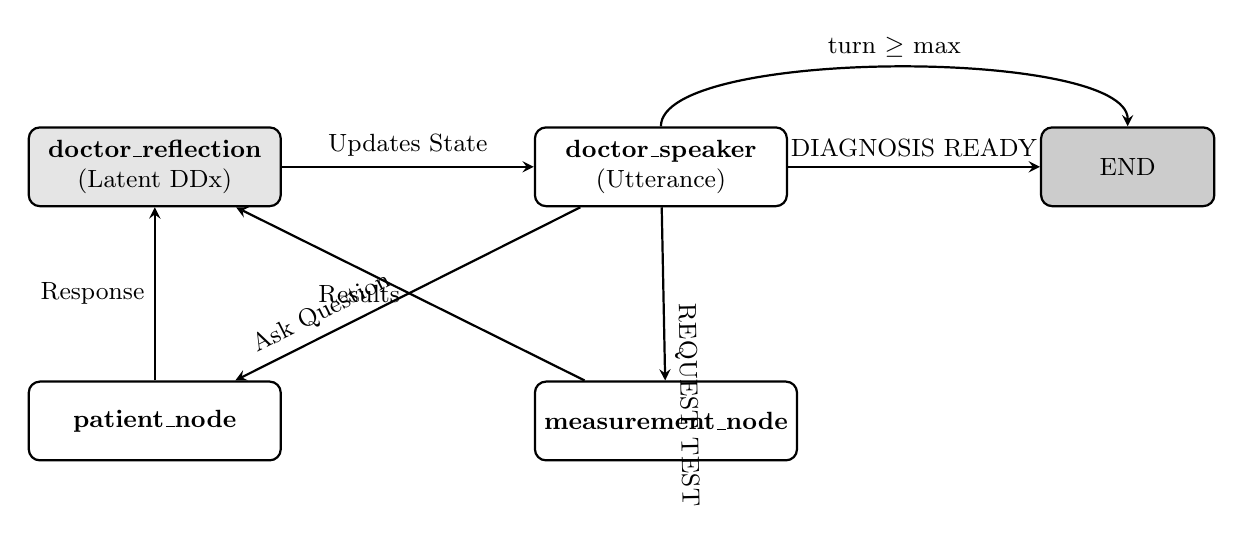
\begin{tikzpicture}[
            node distance=2.2cm and 3.2cm,
            agent/.style={rectangle, rounded corners, draw=black, thick,
                          minimum width=3.2cm, minimum height=1cm, align=center, font=\small},
            hidden/.style={rectangle, rounded corners, draw=black, fill=gray!20, thick,
                           minimum width=3.2cm, minimum height=1cm, align=center, font=\small},
            terminal/.style={rectangle, rounded corners, draw=black, fill=gray!40, thick,
                             minimum width=2.2cm, minimum height=1cm, align=center, font=\small},
            arrow/.style={thick, ->, >=stealth}
        ]
        \node[hidden] (reflection) {\textbf{doctor\_reflection} \\ (Latent DDx)};
        \node[agent, right=of reflection] (speaker) {\textbf{doctor\_speaker} \\ (Utterance)};
        \node[agent, below left=of speaker] (patient) {\textbf{patient\_node}};
        \node[agent, below right=of reflection] (measurement) {\textbf{measurement\_node}};
        \node[terminal, right=of speaker] (end) {END};
        
        \draw[arrow] (reflection) -- node[above, font=\small]{Updates State} (speaker);
        \draw[arrow] (speaker) -- node[above right, sloped, font=\small]{REQUEST TEST} (measurement);
        \draw[arrow] (speaker) -- node[above left, sloped, font=\small]{Ask Question} (patient);
        \draw[arrow] (speaker) -- node[above, font=\small]{DIAGNOSIS READY} (end);
        \draw[arrow] (speaker.north) .. controls +(up:1cm) and +(up:1cm) ..
            node[above, font=\small]{turn $\geq$ max} (end.north);
        \draw[arrow] (patient) -- node[left, font=\small]{Response} (reflection);
        \draw[arrow] (measurement) -- node[left, font=\small]{Results} (reflection);
        \end{tikzpicture}
        }
    \end{figure}
\end{frame}

% Slide 12: Process-Oriented Clinical Metrics
\begin{frame}{Process-Oriented Clinical Metrics}
    To evaluate \textit{how} a model reasons, terminal accuracy is insufficient. We formulated three process-based metrics:
    \vspace{0.3cm}
    \begin{itemize}
        \item \textbf{Diagnostic Stability (DS):} Measures hypothesis "thrashing." Computed via the average Jaccard similarity of consecutive differential diagnoses across turns. High DS means logical anchoring; low DS implies erratic switching.
        \item \textbf{Test Rationality (TR):} A binary compliance check ensuring foundational, non-invasive investigations (e.g., vitals, CBC) are strictly ordered before advanced/invasive tests (e.g., MRI, biopsy).
        \item \textbf{Information Efficiency (IE):} The ratio of unique differential hypotheses explored per aggregate conversational turn.
    \end{itemize}
\end{frame}

% Slide 13: Structured Cognitive Bias Injections
\begin{frame}{Structured Cognitive Bias Injections}
    Can LLMs mimic dangerous human cognitive errors? We injected ecologically valid distortions into the \texttt{ClinicalState}:
    \vspace{0.3cm}
    \begin{itemize}
        \item \textbf{Recency Bias ($k=5$):} The system injects the histories of the 5 most recently processed simulated cases into the Doctor’s prompt. This mimics a clinician overly influenced by the current emergency room trend, exploiting transformer attention dynamics.
        \item \textbf{Confirmation Bias:} The Doctor is primed with strong, medically plausible but entirely \textit{incorrect} initial hypotheses, testing its susceptibility to \textit{premature diagnostic closure}.
    \end{itemize}
\end{frame}

% Slide 14: Dynamic LoRA Adapter Routing
\begin{frame}{Dynamic LoRA Adapter Routing}
    To resolve catastrophic forgetting (where medical fine-tuning destroys conversational logic), we decouple the model's cognitive resources.
    \vspace{0.3cm}
    \begin{itemize}
        \item \textbf{Approach:} We load a base model (JSL-MedMistral) and train two lightweight Low-Rank Adaptation (LoRA) adapters ($\approx$25 MB each).
        \item \textbf{Reasoning Adapter ($T=0.1$):} Activated strictly during the \texttt{doctor\_reflection} node to enumerate structured differential diagnoses.
        \item \textbf{Dialogue Adapter ($T=0.7$):} Activated strictly during the \texttt{doctor\_speaker} node to preserve empathy and syntactic logic.
        \item \textbf{Inference:} The LangGraph DCG executes a pointer swap between adapters at runtime ($<1$ms latency) depending on the active state constraint.
    \end{itemize}
\end{frame}

% Slide 15: Experimental Accuracy (E1-E3)
\begin{frame}{E1–E3: Baseline \& Foundational Outcomes}
    \textbf{Setup:} 107 MedQA Scenarios, 10 Turns Max.
    \vspace{0.3cm}
    \begin{table}
        \centering
        \begin{tabular}{llcc}
            \toprule
            \textbf{Exp.} & \textbf{Doctor Configuration} & \textbf{Bias} & \textbf{Accuracy (\%)} \\
            \midrule
            E1 & Mistral-7B-v0.2           & None         & 45.6 \\
            E2 & JSL-MedMistral-7B                 & None         & 50.2 \\
            E3 & Llama-3.1-8B-Instruct             & None         & 51.5 \\
            \bottomrule
        \end{tabular}
    \end{table}
    \vspace{0.1cm}
    \textbf{Insights:}
    \begin{itemize}
        \item The introduction of the metacognitive reflection node provided enough structural scaffolding to raise E1 accuracy to 45.6\%, actively compensating for the removal of Lexical Leakage.
        \item Instruction-aligned generalist models (E3) outperform purely medically specialized models (E2) in interactive multi-turn tasks.
    \end{itemize}
\end{frame}

% Slide 16: E6: Dynamic LoRA Results
\begin{frame}{E6: Dynamic LoRA Results}
    \begin{figure}
        \centering
        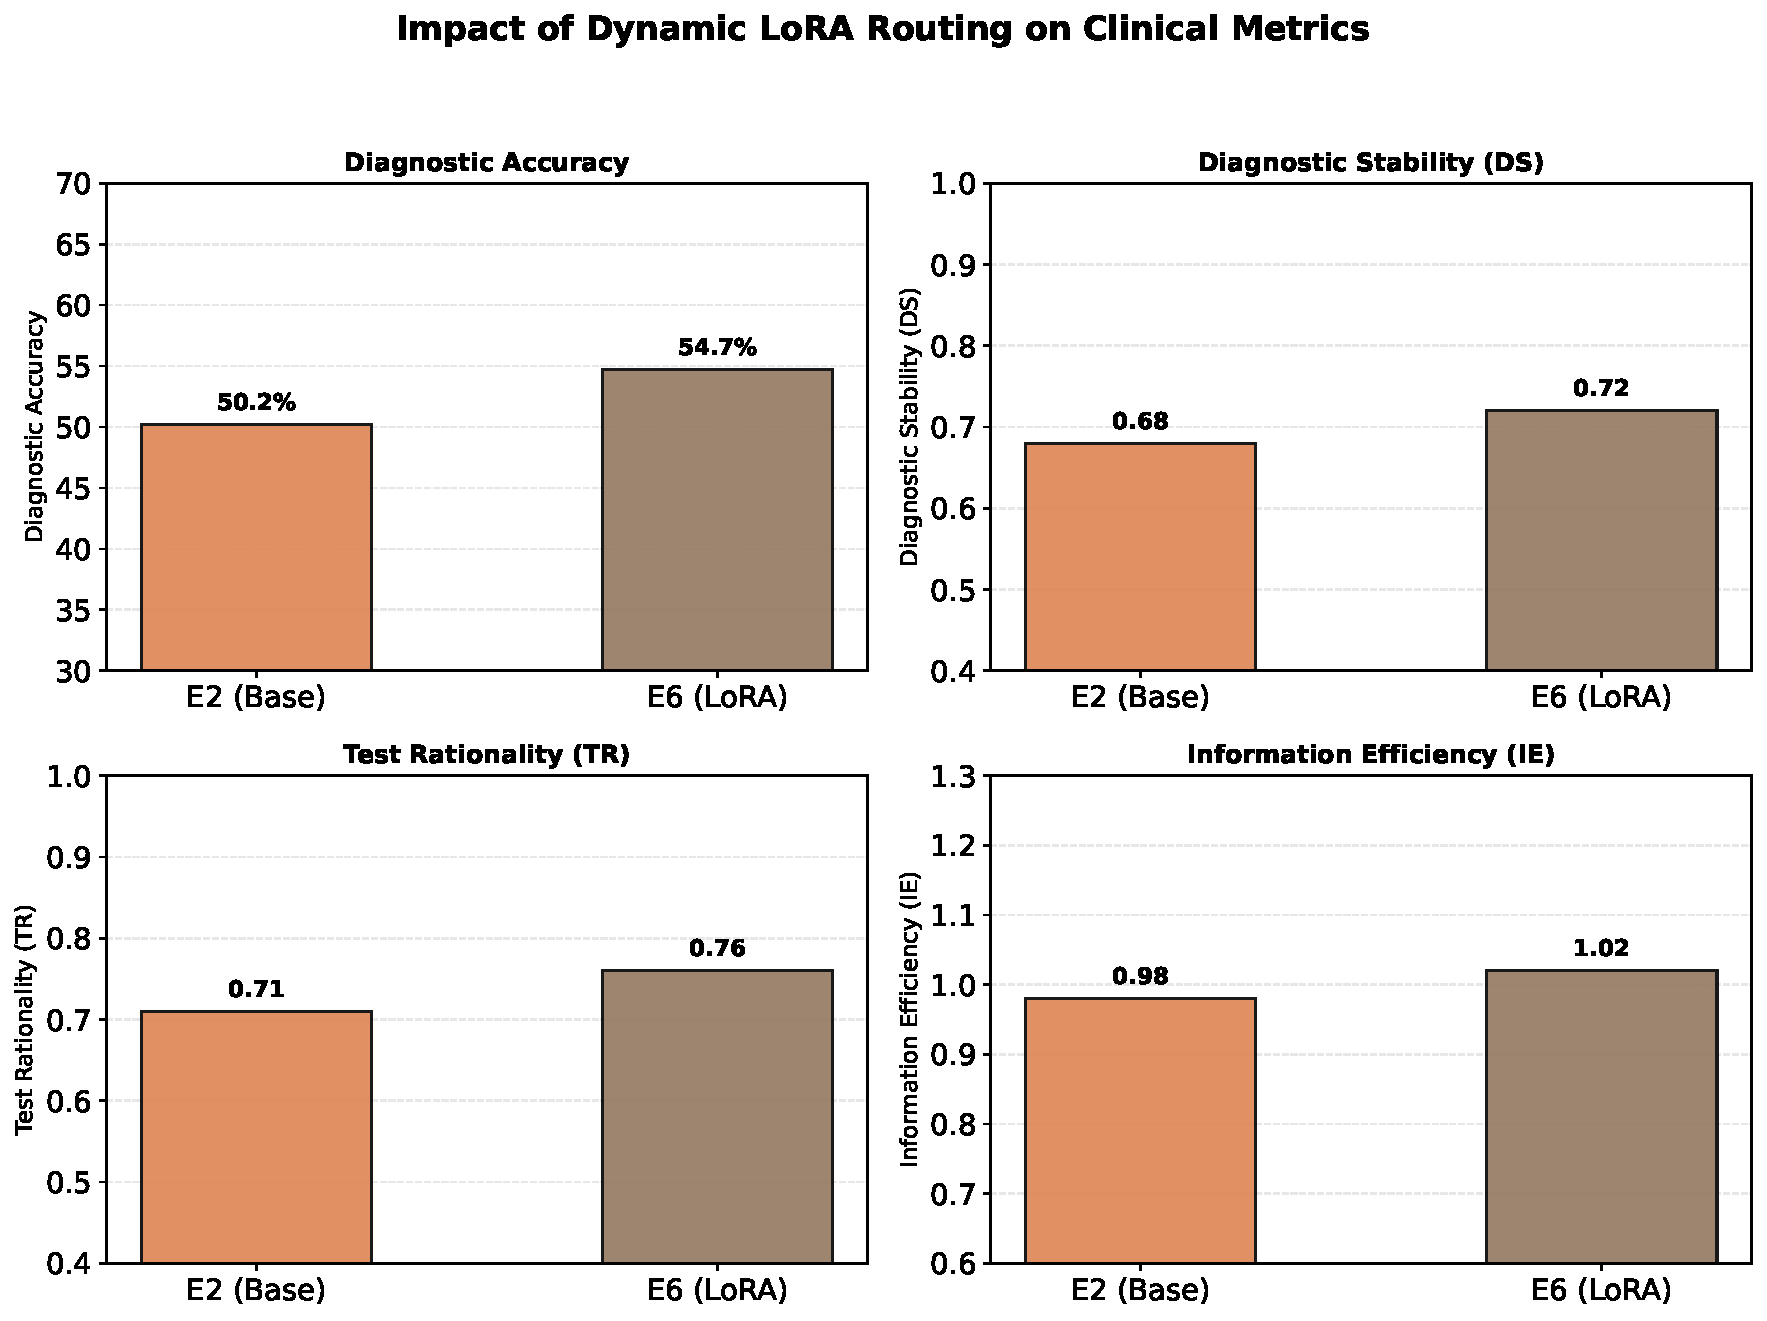
\includegraphics[height=0.45\textheight]{../Final_Report_Humanized/Pictures/lora_comparison.pdf}
    \end{figure}
    \begin{itemize}
        \item \textbf{Highest Overall Accuracy (54.7\%):} The E6 configuration utilizing Dynamic LoRA routing on JSL-MedMistral outperformed all standalone endpoints.
        \item \textbf{Conclusion:} Decoupling medical deduction from conversational dialogue physically at the matrix-adapter layer resolves the specialisation vs. alignment trade-off entirely.
    \end{itemize}
\end{frame}

% Slide 17: Process Metrics \& Safety Threat of Biases
\begin{frame}{The Safety Threat of Cognitive Biases}
    \textbf{Observations from Process-Oriented Measurement:}
    \begin{figure}
        \centering
        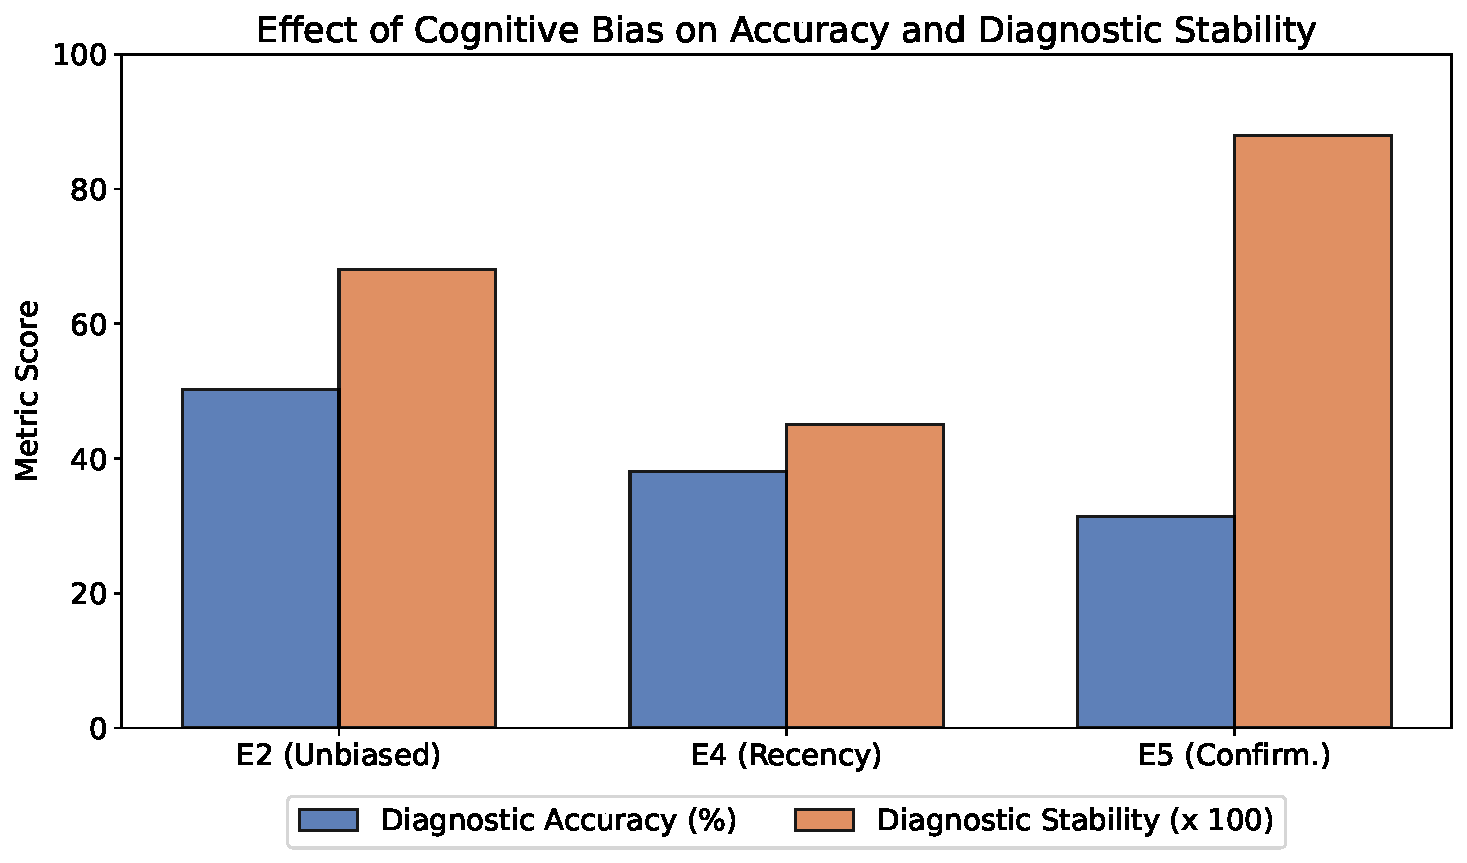
\includegraphics[height=0.35\textheight]{../Final_Report_Humanized/Pictures/bias_combined.pdf}
    \end{figure}
    \begin{itemize}
        \item \textbf{Recency Bias (Accuracy = 38.1\%):} Hypothesis thrashing causes Diagnostic Stability to collapse ($DS = 0.45$).
        \item \textbf{Confirmation Bias (Accuracy = 31.4\%):} The lowest accuracy in the study, yet it presents pathologically high stability ($DS = 0.88$). It rigidly ignores contradictory clinical evidence (premature closure).
    \end{itemize}
\end{frame}

% Slide 18: Discussion - Specialisation vs Alignment
\begin{frame}{Discussion: Specialisation vs Alignment}
    \begin{itemize}
        \item \textbf{The Trade-off is Avoidable:} E6 proves that the traditional tension between domain-specific fine-tuning and generalized instruction following is an artifact of monolithic model updates, not an intrinsic limitation of Large Language Models.
        \item \textbf{Evaluating Process is Mandatory:} Accuracy alone is dangerous. An model exhibiting high terminal accuracy but generating $DS$ metric signatures indicative of premature hypothesis closure is wildly unsafe for real-world deployment.
        \item \textbf{Open-Source Viability:} Local, quantised LLMs orchestrating across a LangGraph topology represent a scalable, highly secure alternative to proprietary, cloud-hosted API ecosystems.
    \end{itemize}
\end{frame}

% Slide 19: Conclusion
\begin{frame}{Conclusion}
    \begin{itemize}
        \item \textbf{AgentClinic v2} successfully moves clinical AI evaluation away from static factual recall and towards dynamic, trajectory-aware simulation.
        \item Implemented heterogeneous multi-engine isolation to resolve the mathematically proven Lexical Leakage vulnerability.
        \item The introduction of the \textbf{Latent Metacognitive Reflection Node} makes LLM reasoning observable and quantifiable.
        \item While open-source models achieved peaks of \textbf{54.7\%} diagnostic accuracy (E6 Dynamic LoRA), their severe susceptibility to confirmation and recency bias indicates they are \textbf{not yet ready} for direct, unmonitored clinical deployment. 
    \end{itemize}
\end{frame}

% Slide 20: Future Work
\begin{frame}{Future Work}
    The AgentClinic v2 framework serves not merely as an evaluator, but as an advanced foundation for post-training alignment:
    \vspace{0.3cm}
    \begin{itemize}
        \item \textbf{Direct Preference Optimisation (DPO):} We propose deploying a Process Reward Model. By heavily punishing consultation paths exhibiting low Test Rationality, DPO can actively train the LLM's behavioral policy to prefer systematic, guideline-concordant reasoning sequences over premature guessing.
        \item \textbf{Self-Play AI Feedback:} Eliminating human-annotation dependency. By employing AgentClinic as an automated Reinforcement Learning environment, heterogeneous clinical agents can autonomously generate thousands of synthetic consultation trajectories, using $DS$ and $TR$ process outcomes as reward signals.
    \end{itemize}
\end{frame}

\end{document}
